\subsection{Time Limit Experiments Results}
%
%\subsection{Accuracy evaluation}
The dataset used is $Flight$ database for flight delays in year 2008 obtained from The U.S. Department of Transportation's Bureau of Transportation Statistics (BTS) with size 250 K tuples \footnote { http://www.transtats.bts.gov/}. The dataset 
contains 10 dimension attributes and 10 measures attributes with 
we run this experiment on SeeDB 
over \emph{All} aggregate functions \emph{Count, Sum, Average, Min, and Max} with 
a space size=$5 \times 10 \times 10=500$ views and 
the deviation metric is Earth Movers Distance (EMD). All Experiments were executed 5 times and obtained the averaged results, we concerned with evaluating the 
performance and the efficiency of the proposed algorithms along different time limits $tl$ and various sets of top deviated views $K$. In experiments, the analyst
posed a query\\
 $Q:$ select * from ontime2008 where dimmonth in('APR','MAY','JUN') \\ to compare the second quarter's dataset with the entire dataset and run to find different $K$ views while varying time limits. In addition we evaluated the quality of the results of $top-K$ views produced by each algorithm with those produced by SeeDB baseline e.g. without time limits or any optimizations used and the average SeeDB baseline execution time is 23200ms. 
we implement $SeeDB_Timelimit$ strategy which processes the entire data and views in a specified execution time limit and it recommends top views that processed in that time limit.
This strategy gives a lower bound on accuracy and upper bound
on error distance: for any proposed technique should be useful. 
%\mas{for all plots - use shades of grey, use one axis, use one metric per plot, and use straight lines not curves!}
\\ In figures \ref{fig:tlfig1} and \ref{fig:tlfig11} show the accuracy and distance error of the results produced by
algorithms $Sela$ , $Diff_DVal$, $DimHisto$, and $SeeDB_Timelimit$ to find a top $(K=100)$ views compared with SeeDB baseline on different execution time limits. These algorithms outputs an ordered set
of dimension attributed based on their priorities and submit the ordered set to execution engine $SeeDB_Timelimit$ then it processes all views generated according to the ordered set that produced by algorithms.
%\mas{and how did these algorithms become aware of the time limit?}
As shown, $SeeDB_Timelimit$ shows high distance error and very low accuracy as well while the algorithms $Sela$ and $Diff_DVal$ scored higher accuracy than 
$DimHisto$. Although the proposed algorithms show a growing in accuracy while extending the time limit but they achieved 100\% accuracy from time limit 18000ms. The 
algorithms boasted the performance more than 30\% and preserved the quality of views. In the other side, figure \ref{fig:tlfig2} describes the execution costs referred as overhead time of 
the proposed algorithms on the same experiment. $DimHisto$ algorithm execution time is about 1200ms while the algorithms $Sela$ and $N-N'$ have almost the similar 
execution time about 825ms. 
%\mas{is that overhead time or total time?!} 
This shows that $Sela$ and $Diff_DVal$ algorithms are faster 66 \% than $DimHisto$ algorithm. As discussed previously the additional histograms distance computations caused the extra overhead algorithm $DimHisto$. 

\begin{figure}
  \begin{subfigure}[b]{0.32\textwidth}
    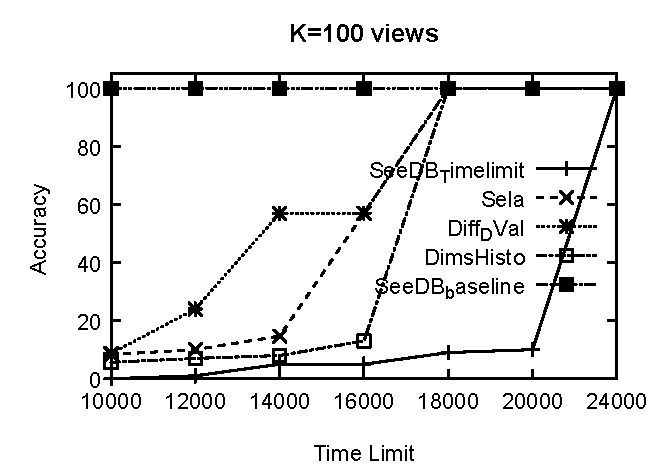
\includegraphics[width=\textwidth]{tl1.pdf}
    \caption{Accuracy}
        \label{fig:tlfig1}%
  \end{subfigure}
	\begin{subfigure}[b]{0.32\textwidth}
    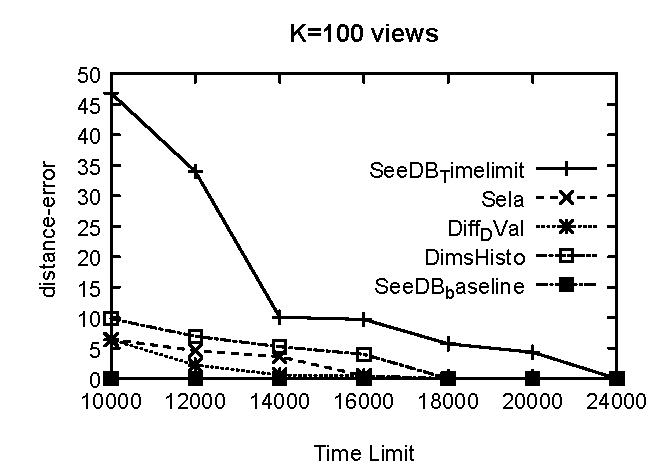
\includegraphics[width=\textwidth]{tl11.pdf}
    \caption{Distance-error}
        \label{fig:tlfig11}%
  \end{subfigure}
  %
  \begin{subfigure}[b]{0.32\textwidth}
    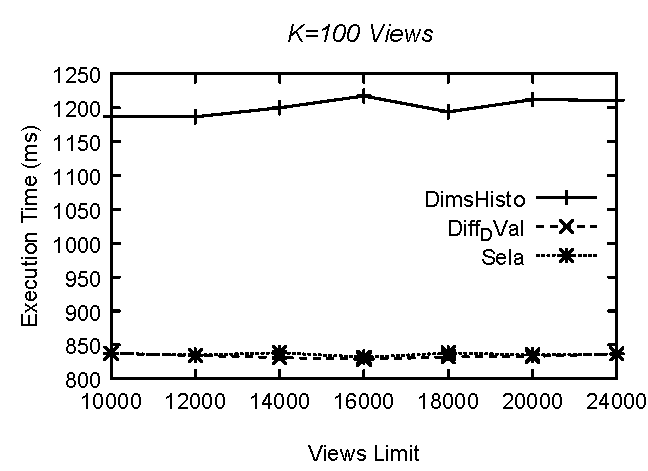
\includegraphics[width=\textwidth]{tl2.pdf}
     \caption{Execution times}
        \label{fig:tlfig2}
  \end{subfigure}
  \caption{Performance of Algorithms $Sela$ , $Diff_DVal$, $DimHisto$, and $SeeDB_Timelimit$ on different time limits}
\end{figure}

 %\begin{figure}[h]
%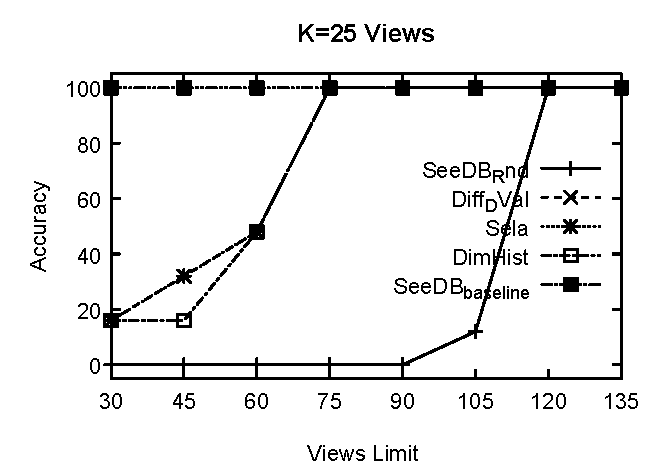
\includegraphics[width=\textwidth]{21.pdf}
%\caption{Accuracy compared with  the view space size for the Algorithms $Sela$ , $N-N'$, $DimHisto$, and $SeeDB_Rnd$}
%\label{fig:fig1}%
%\end{figure}



%\begin{figure}[h]
%\includegraphics[width=\textwidth]{{22.pdf}}
%\caption{Error Distance according to the view space size for the Algorithms $Sela$ , $N-N'$, $DimHisto$, and $SeeDB_Rnd$}
%\label{fig:figa2}%
%\end{figure}

  
%  \begin{figure}[h]
%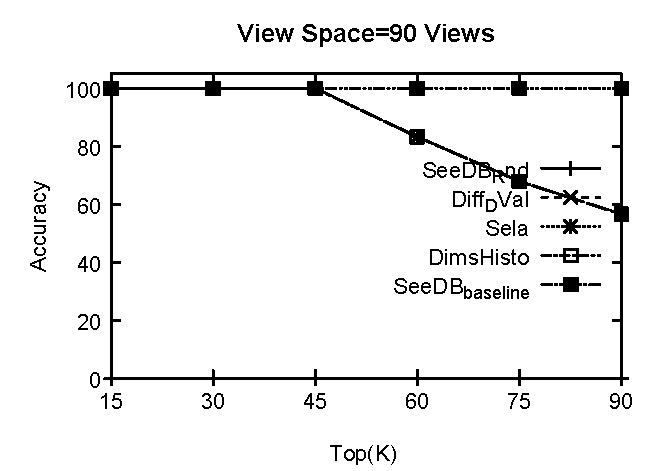
\includegraphics[width=\textwidth]{11.pdf}
%\caption{Accuracy compared with  top(K) views for the Algorithms $Sela$ , $N-N'$, $DimHisto$, and $SeeDB_Rnd$}
%\label{fig:fig3}%
%\end{figure}

\begin{figure}
  \begin{subfigure}[b]{0.32\textwidth}
    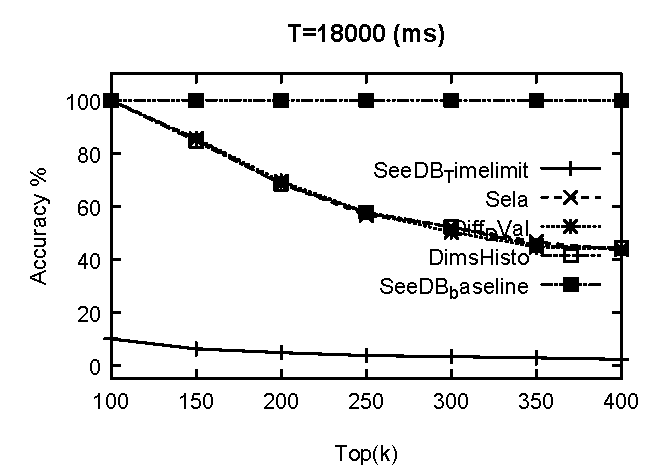
\includegraphics[width=\textwidth]{tl3.pdf}
    \caption{Accuracy }
       \label{fig:tlfig3}
  \end{subfigure}
	\begin{subfigure}[b]{0.32\textwidth}
    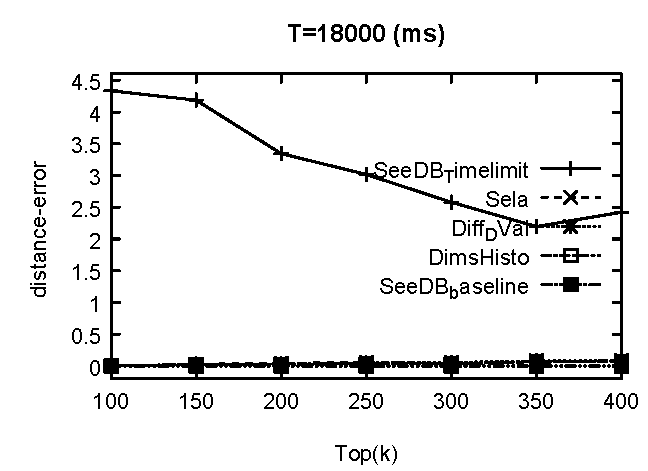
\includegraphics[width=\textwidth]{tl31.pdf}
    \caption{A Distance-error}
       \label{fig:tlfig31}
  \end{subfigure}
  %
  \begin{subfigure}[b]{0.32\textwidth}
    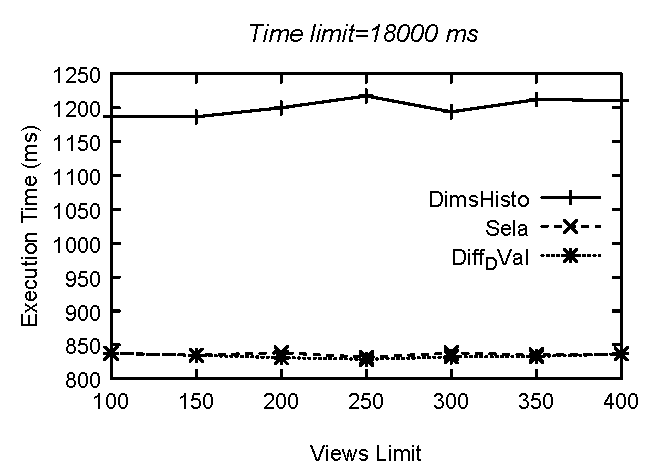
\includegraphics[width=\textwidth]{tl4.pdf}
     \caption{Execution times}
       \label{fig:tlfig4}%
  \end{subfigure}
  \caption{ Performance of Algorithms $Sela$ , $Diff_DVal$, $DimHisto$, and $SeeDB_Timelimit$ on varying top(K) views}
\end{figure}

In figures \ref{fig:tlfig3} and \ref{fig:tlfig31} show the accuracy of the 
algorithms $Sela$ , $N-N'$, $DimHisto$, and $SeeDB_Timelimit$ in a certain time limit $tl=18000$ ms
 comparing with different sets of top(k) views as shown all algorithms scored 100\% accuracy in the first top 100 views. 
However, The accuracy declines with the increasing top(K) in a fixed time limit but the 
proposed algorithms scored very small distance error for large sets of top(K) while $SeeDB_Timelimit$ shows very low accuracy and huge distance error. 
As illustrated in \ref{fig:tlfig2} The execution costs of the proposed algorithms remains stable on different time limits and it shows
the similar behavior figure \ref{fig:tlfig4} the overhead is fixed along different top-k views.\\
  
To sum up, the proposed algorithms improved the quality of results according two the evaluation metrics that used along different
K sizes and various times limits. Moreover, the algorithms overhead is comparatively small with the total execution of SeeDB baseline.	
%\begin{figure}[t]
%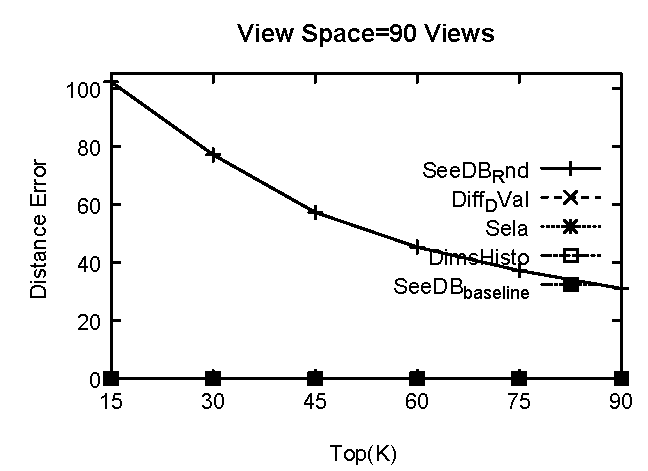
\includegraphics[width=\textwidth]{12.pdf}
%\caption{Error Distance compared with  the view space size for the Algorithms $Sela$ , $N-N'$, $DimHisto$, and $SeeDB_Rnd$}
%\label{fig:fig4}%
%\end{figure}
